\section{Issue 135: Uploading images from phone}

Issue 135 was to implement a feature allowing users to upload pictures from their phone/tablet to the the pictogram database. The feature was described as a userstory with the following description: "As a guardian, I would like a way to add pictograms by choosing an image from my phone gallery so that I can quickly improvise if the system does not have the activity I want." 
Initially we expected the feature to require a new screen and a new \gls{bloc} for handling communication with the api. We started out by designing the view, since the view should contain as little logic as possible the \gls{ui} should not have any influence on how the logic will be implemented. The \gls{ui} also served as a skeleton to implement and test the functionality while developing the final screen can be seen in \autoref{fig:uploadScreen}.

\begin{figure}[!h]
  \centering
  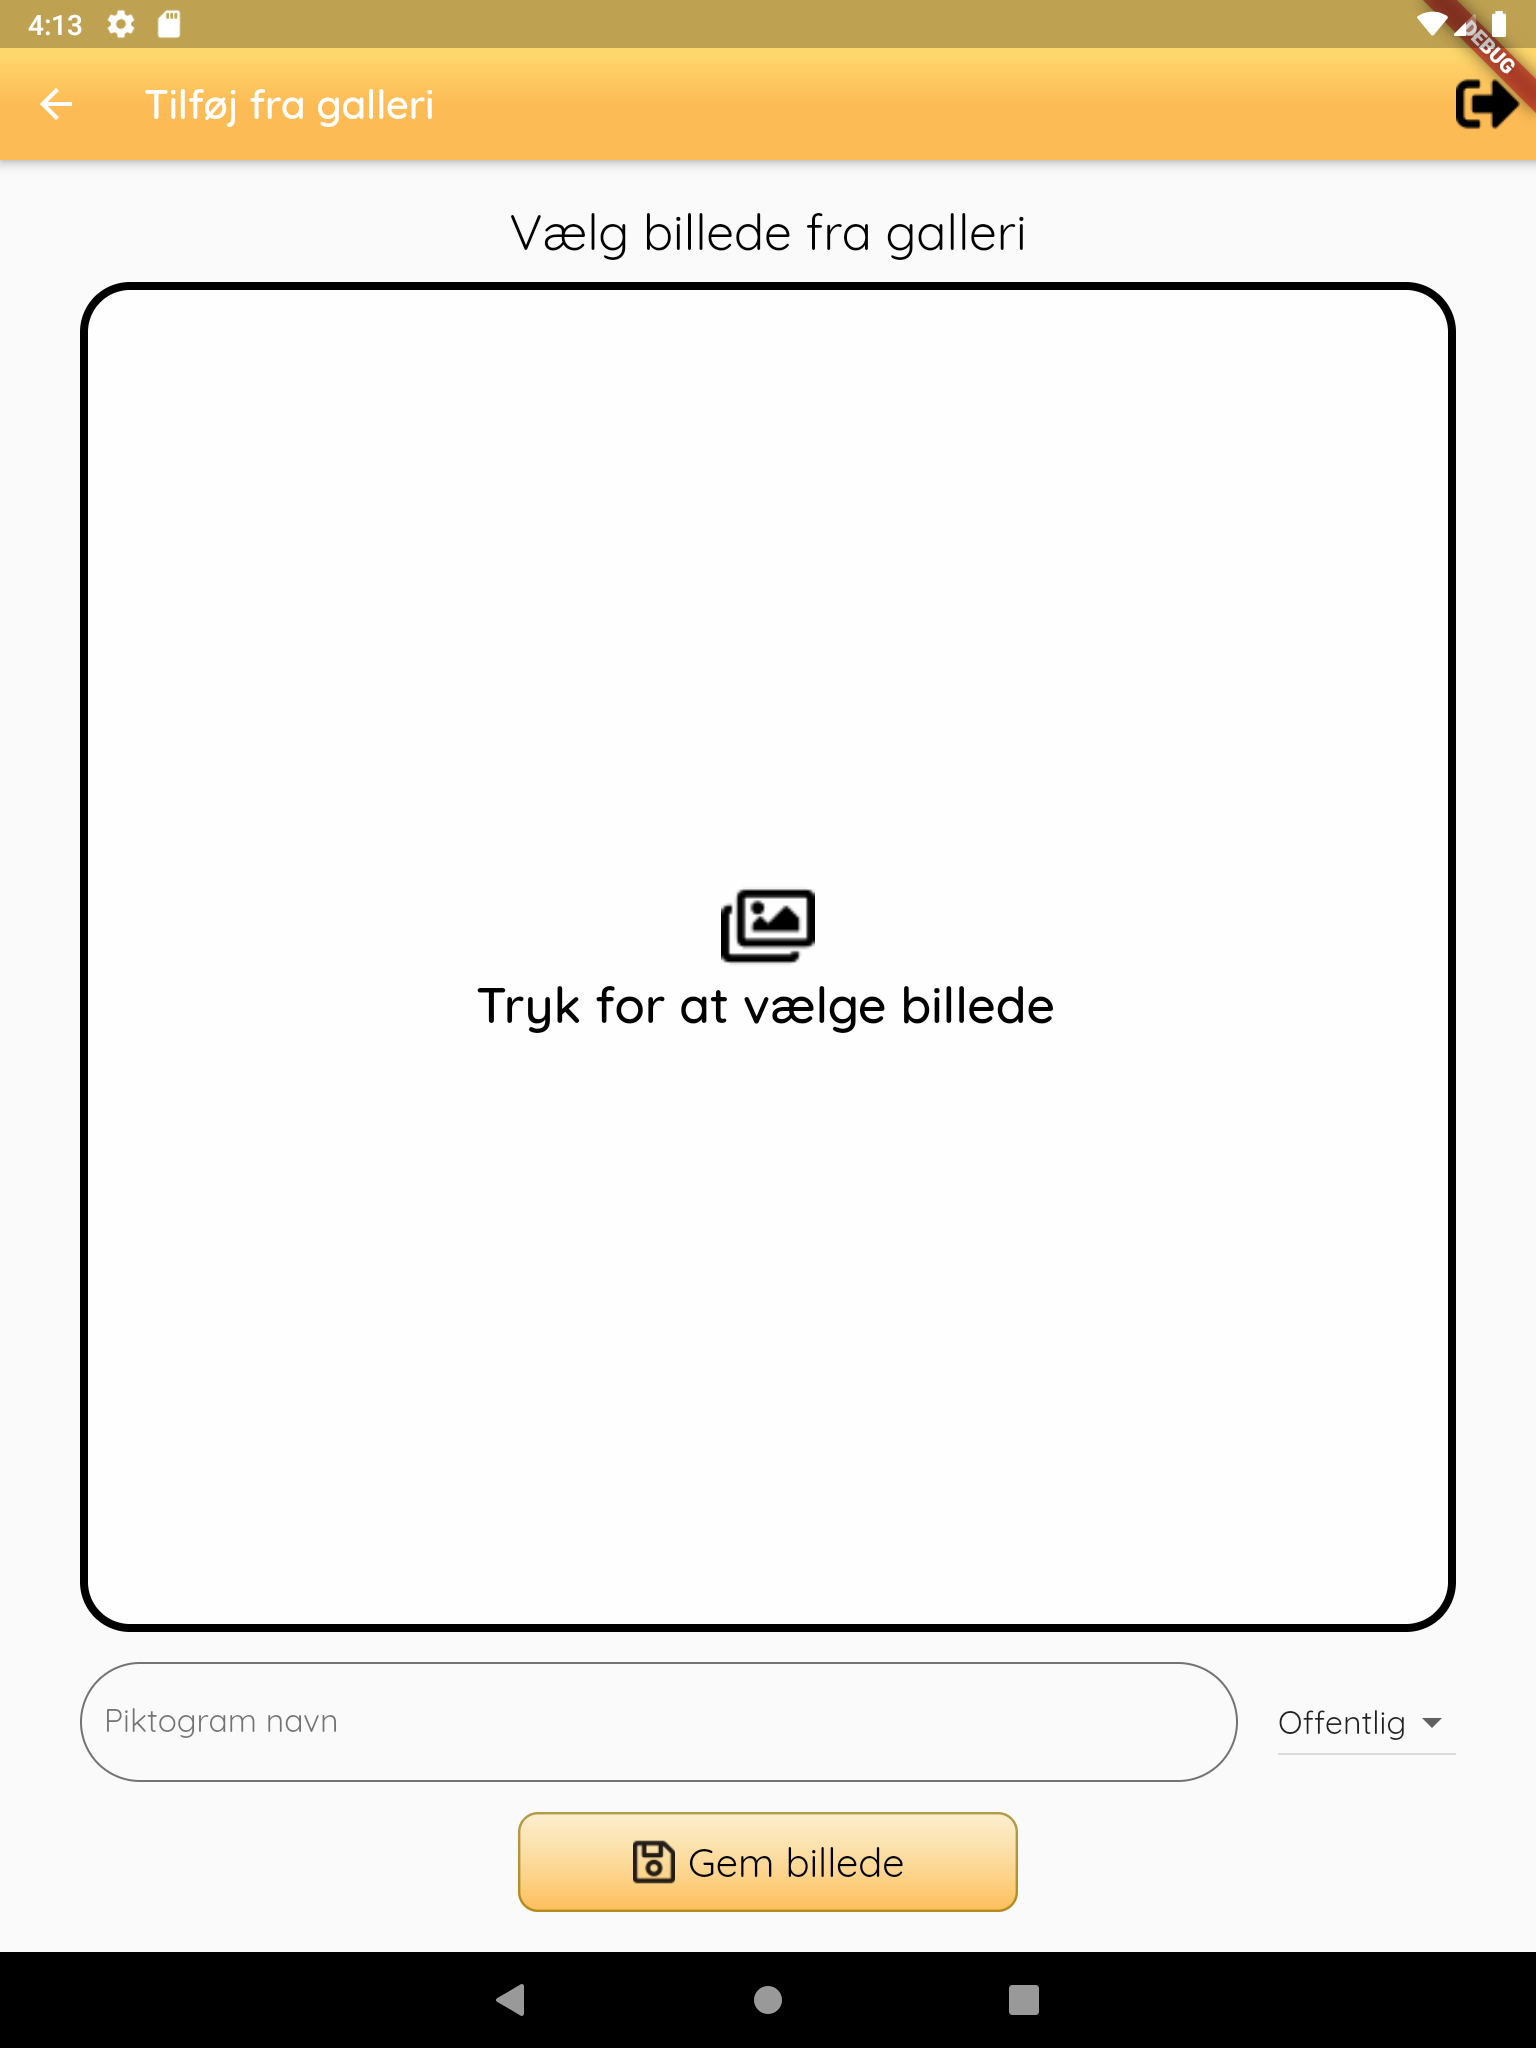
\includegraphics[width=0.7\textwidth]{figures/uploadPictogramScreen.png}
  \caption{Screenshot of the final implementation of the upload image screen}
  \label{fig:uploadScreen}
\end{figure}

For implementing the functionality of grabbing the image from the phone, a plugin was used, without any issues.
For uploading the image to the database we ran into many troubles, both in the \gls{fapi} 